\documentclass[11pt]{article}
\usepackage[letterpaper,margin=1in]{geometry}
\usepackage[T1]{fontenc}
\usepackage[utf8]{inputenc}
\usepackage{graphicx}
\usepackage{amsmath}
\usepackage{booktabs}
\usepackage{caption}
\usepackage{float}
\usepackage{enumitem}
\usepackage[hidelinks]{hyperref}
\captionsetup{font=small,labelfont=bf,skip=4pt}
\setlength{\textfloatsep}{8pt}\setlength{\intextsep}{8pt}
\setlist{itemsep=2pt,topsep=4pt}
\setlength{\parskip}{4pt}
\newcommand{\note}[1]{\par\vspace{2pt}{\raggedright\footnotesize\textit{Note:} #1\par}}

\title{\vspace{-1.8cm}\Large Will Rising Unemployment Push Up Consumer Loan Delinquency?\\[2pt]
\large Early Warning Signals and the Fed's 2026 Stress Scenarios}
\author{Farida Issifou -- University of Neuchâtel -- Date: October 27, 2026}
\date{}

\begin{document}
\maketitle
\vspace{-1cm}

\begin{abstract}
\noindent This note asks whether following the labour market gives lenders and supervisors an earlier and more accurate warning of rising consumer loan delinquency in the United States, and what the Federal Reserve's 2026 stress scenarios would mean for delinquency. Using quarterly data from 1987 to 2025, I compare forecasts based only on the past of delinquency with forecasts that also use unemployment. I find three things. First, unemployment does not give an earlier warning: in real time it does not improve forecasts one to four quarters ahead. Second, it is useful for scenario analysis: each additional point of unemployment raises delinquency by about 0.15 points. Third, under the Fed's severely adverse scenario, delinquency would rise from 2.6\% to about 3.3\% in 2027 through job losses alone, and to around 3.9\% once a housing and credit shock similar to 2008 is taken into account.
\end{abstract}

\section*{Why Consumer Loan Delinquency Matters}

The delinquency rate measures the share of consumer loans (credit cards, car loans and other personal loans) held by US commercial banks on which borrowers are at least 30 days late with their payments. It is one of the first signs of financial stress in households, and it comes before the losses banks have to write off. Lenders use it to set aside provisions against future losses, and supervisors use it to judge whether banks hold enough capital to survive a recession.

This analysis uses quarterly data from the Federal Reserve Bank of St.\ Louis (FRED), from the first quarter of 1987 to the last quarter of 2025. Figure~\ref{fig:history} shows that delinquency and unemployment usually rise together in recessions. The 2008 crisis is the clearest case, with delinquency reaching a record 4.85\% in 2009. The COVID-19 recession is the exception: unemployment jumped to 13\% in 2020 while delinquency fell to its lowest level on record in 2021, because stimulus payments and loan forbearance allowed households to keep paying or to pause payments without being counted as late (Cherry et al., 2021). After rising again in 2023 and 2024, delinquency reached 2.62\% at the end of 2025.

\begin{figure}[htbp]
\centering
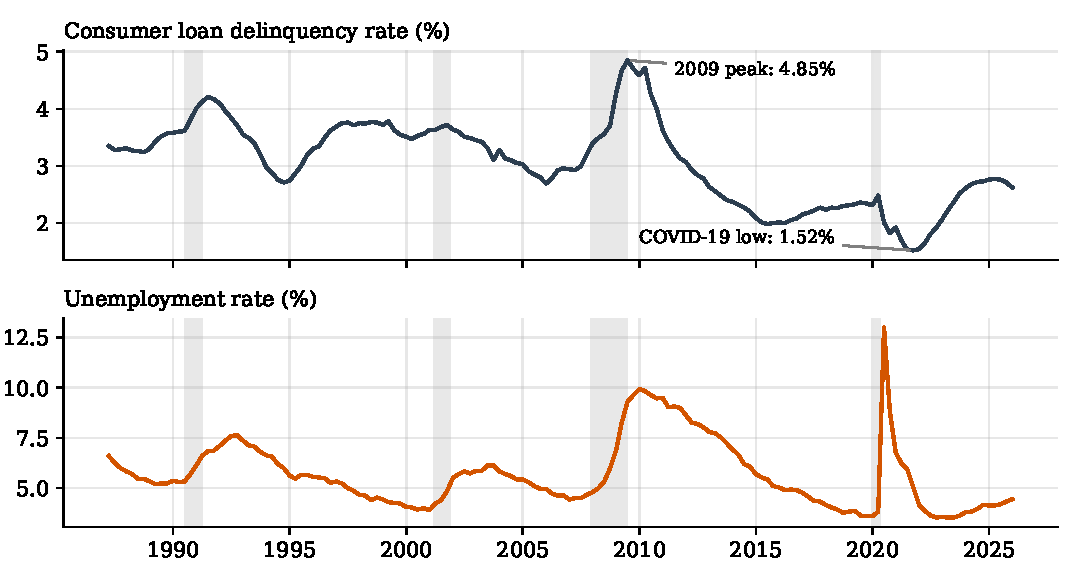
\includegraphics[width=0.8\textwidth]{figures/history.pdf}
\caption{Consumer loan delinquency and unemployment in the United States, 1987--2025}
\label{fig:history}
\note{Quarterly averages. Shaded areas are US recessions (NBER dates). Source: FRED, series DRCLACBS and UNRATE.}
\end{figure}

\section*{Does the Labour Market Give an Earlier Warning?}

To answer this question, I compare two kinds of forecast. The first uses only the past behaviour of delinquency: when it has been rising, it tends to keep rising for a while. The second adds the change in unemployment, which was the only economic indicator to show a clear link with delinquency in the earlier steps of the project. The interest rate, consumer confidence and the shape of the yield curve add nothing once unemployment is included. Starting in 2005, both models are estimated again every quarter on the data available at that time, and asked to forecast delinquency one to four quarters ahead. Comparing these forecasts with what actually happened shows which model would have warned us better.

The answer is that the labour market does not provide an earlier warning. When the future path of unemployment has to be forecast as well, which is the situation lenders face in practice, the model with unemployment is no more accurate than the one based on delinquency alone: a year ahead, both miss the actual rate by about 0.41 points on average (Table~\ref{tab:accuracy} in the appendix). There are two reasons for this. Unemployment moves in the same quarter as delinquency or one quarter before, so it gives little lead time. And forecasting unemployment is as hard as forecasting delinquency itself.

Even when the model is given the true path of unemployment, the gain is small. It is largest in the 2008--2010 crisis, where the error a year ahead falls by 14\%, but even then the error stays three times larger than in normal years, and the improvement is not statistically significant. In 2020 the model with unemployment performs much worse, since it predicts a surge in delinquency that never came.

\section*{What the Fed's 2026 Stress Scenarios Imply}

The unemployment model is more useful for a different question: \emph{what happens to delinquency if unemployment follows a given path?} This is exactly what a stress test asks. In the model, each additional point of unemployment raises delinquency by about 0.15 points over two quarters, and the effect lasts until unemployment falls again (Table~\ref{tab:coef} in the appendix). This is in line with research showing that losing a job, rather than a choice not to pay, is the main reason households fall behind on their debts (Gerardi et al., 2018).

In February 2026 the Federal Reserve published the two scenarios used in this year's stress test of large banks (Board of Governors of the Federal Reserve System, 2026). In the \emph{baseline}, unemployment stays near 4.5\% and edges down to 4.2\% by early 2029. In the \emph{severely adverse} scenario, a severe global recession raises unemployment to a peak of 10\% in the third quarter of 2027, and house prices fall by about 30\%. Figure~\ref{fig:scenarios} shows what these paths imply for delinquency.

\begin{figure}[htbp]
\centering
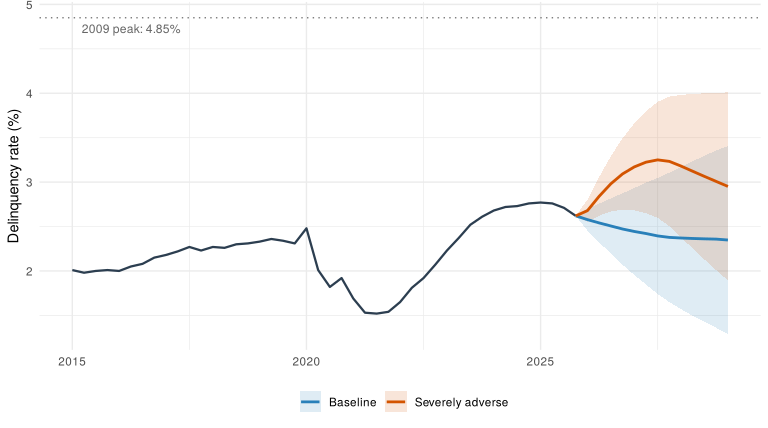
\includegraphics[width=0.78\textwidth]{figures/scenarios.png}
\caption{Consumer loan delinquency under the Fed's 2026 stress scenarios, 2026--2029}
\label{fig:scenarios}
\note{Forecasts from the unemployment model, given the unemployment path of each scenario. Shaded areas are 80\% prediction intervals. The dotted line marks the 2009 record. Quarterly values are in Table~\ref{tab:scenarios} in the appendix.}
\end{figure}

Under the baseline, delinquency continues its slow decline to about 2.35\% in early 2029. Under the severely adverse scenario, it rises to a peak of 3.25\% in the third quarter of 2027, 0.86 points above the baseline, and is still close to 3\% at the end of the scenario.

This peak is likely too low. The scenario combines job losses with a large fall in house prices, a mix close to the 2008 crisis. To see how much of such a crisis the unemployment channel captures, I gave the model the actual rise in unemployment from mid-2007 onwards (Figure~\ref{fig:check2008} in the appendix). It explains 0.81 of the 1.65-point rise in delinquency, about half (49\%), and it starts rising too late, because the crisis began in mortgage and consumer credit before it reached the labour market. If the unemployment channel again accounts for about half of the total, the 0.63-point rise in the severely adverse scenario would become about 1.3 points, for a peak near 3.9\%. This is a rise comparable to 2008, but from a lower starting point, so it stays below the 2009 record.

\section*{Key Takeaways}

For lenders and supervisors, the results point to four messages:
\begin{itemize}
\item \textbf{Watch delinquency itself.} The recent trend of delinquency gives as good an early warning as the labour market. Unemployment data do not add lead time.
\item \textbf{Use unemployment for scenario analysis.} A rule of thumb of about 0.15 points of delinquency per point of unemployment is a simple way to translate a recession scenario into credit stress.
\item \textbf{Treat this as a lower bound.} When a scenario also includes a housing or credit shock, the unemployment channel alone can miss about half of the rise. For the Fed's severely adverse scenario, a range of 3.3\% to 3.9\% at the peak is more prudent than a single number.
\item \textbf{Policy support can break the link.} COVID-19 showed that stimulus and forbearance can keep delinquency low even when unemployment surges. The scenario results assume no such support.
\end{itemize}

This analysis relies on one national series for all consumer loans and on a simple model. Future work could test whether credit-side indicators, such as banks' lending standards or the share of borrowers moving into delinquency, give the early warning that unemployment does not, and whether the results differ between credit cards and car loans.

\section*{References}
\begin{list}{}{\leftmargin=1.5em \itemindent=-1.5em \itemsep=3pt}
\item Board of Governors of the Federal Reserve System (2026). \emph{2026 Final Supervisory Stress Test Scenarios}. Washington, DC, February 4, 2026.
\item Cherry, S., Jiang, E., Matvos, G., Piskorski, T., and Seru, A. (2021). Government and Private Household Debt Relief during COVID-19. \emph{Brookings Papers on Economic Activity}, Fall 2021.
\item Federal Reserve Bank of St.\ Louis (2026). Federal Reserve Economic Data (FRED). Series DRCLACBS, UNRATE, T10Y2Y, FEDFUNDS and UMCSENT.
\item Gerardi, K., Herkenhoff, K. F., Ohanian, L. E., and Willen, P. S. (2018). Can't Pay or Won't Pay? Unemployment, Negative Equity, and Strategic Default. \emph{The Review of Financial Studies}, 31(3):1098--1131.
\end{list}

\newpage
\section*{Appendix}

\subsection*{A. Data and Method}

All series come from FRED and are averaged to quarterly frequency (1987 Q1 to 2025 Q4). Delinquency (DRCLACBS) is the target. The candidate predictors are the unemployment rate (UNRATE), the federal funds rate (FEDFUNDS), consumer confidence (UMCSENT) and the yield spread between 10-year and 2-year Treasury bonds (T10Y2Y). Augmented Dickey-Fuller tests led me to use the yield spread in levels and the other predictors in first differences. Canova-Hansen tests found no seasonality.

The benchmark is an ARIMA(1,1,1) model for delinquency, which forecast better than a naive forecast and than an ARMA in levels. The macro models keep the same dynamics and add predictors:
\[
\Delta \text{dlq}_t = \beta_0\, \Delta u_t + \beta_1\, \Delta u_{t-1} + \text{ARMA}(1,1) \text{ error},
\]
where $\text{dlq}$ is the delinquency rate and $u$ the unemployment rate (Model U). Model U + S adds the yield spread of the previous quarter. Both models include dummies for 2020 Q2 to 2021 Q1, so that the COVID-19 support period does not distort the estimated link between unemployment and delinquency. The full code is available at \url{https://github.com/FaridaISSIFOU/consumer-delinquency-forecasting}.

\begin{table}[H]
\centering
\caption{Estimated effects on the quarterly change in delinquency}
\label{tab:coef}
\small
\begin{tabular}{llccc}
\toprule
Model & Variable & Coefficient & Std.\ error & p-value \\
\midrule
U & $\Delta$ unemployment, same quarter & 0.078 & 0.044 & 0.074 \\
U & $\Delta$ unemployment, previous quarter & 0.075 & 0.040 & 0.062 \\
U & \textbf{Total effect of unemployment} & \textbf{0.153} & & \textbf{0.003} \\
\midrule
U + S & $\Delta$ unemployment, same quarter & 0.069 & 0.041 & 0.090 \\
U + S & $\Delta$ unemployment, previous quarter & 0.078 & 0.039 & 0.046 \\
U + S & Yield spread, previous quarter & $-0.059$ & 0.015 & 0.000 \\
\bottomrule
\end{tabular}
\note{Estimation sample 1988 Q2 to 2025 Q4 (151 quarters), ARMA(1,1) errors. COVID-19 dummies are not shown. Each unemployment coefficient is borderline on its own because the two quarters are correlated, but their sum is clearly significant. The negative sign of the yield spread reflects the Fed's reaction to credit stress (rate cuts steepen the curve when delinquency starts to recover), which is why Model U + S is not used for the stress scenarios.}
\end{table}

\begin{table}[H]
\centering
\caption{Forecast accuracy, 2005--2025: average error (RMSE, percentage points)}
\label{tab:accuracy}
\small
\begin{tabular}{lcccc}
\toprule
 & \multicolumn{4}{c}{Quarters ahead} \\
\cmidrule(lr){2-5}
Model & 1 & 2 & 3 & 4 \\
\midrule
\multicolumn{5}{l}{\textit{Real time: future unemployment is forecast}} \\
Delinquency only, ARIMA(1,1,1) & 0.113 & 0.213 & 0.315 & 0.411 \\
Model U & 0.112 & 0.215 & 0.319 & 0.417 \\
Model U + S & 0.110 & 0.210 & 0.315 & 0.413 \\
\midrule
\multicolumn{5}{l}{\textit{Known path: actual future unemployment is used}} \\
Model U & 0.112 & 0.213 & 0.317 & 0.405 \\
Model U + S & 0.109 & 0.206 & 0.304 & 0.383 \\
\bottomrule
\end{tabular}

\vspace{6pt}
\begin{tabular}{lccc}
\toprule
4 quarters ahead, by period & Normal periods & 2008--2010 crisis & COVID-19 recovery \\
\midrule
Delinquency only, ARIMA(1,1,1) & 0.201 & 0.805 & 0.456 \\
Model U (known path) & 0.193 & 0.774 & 0.543 \\
Model U + S (known path) & 0.220 & 0.696 & 0.493 \\
\bottomrule
\end{tabular}
\note{Rolling-origin forecasts: each model is re-estimated every quarter from 2004 Q4 on the data available at that time. Forecasts that target the emergency support period (2020 Q2 to 2021 Q4) are excluded, since no stress scenario assumes such support. Including them, the macro models are much worse than the benchmark (0.22 against 0.13 one quarter ahead). Diebold-Mariano tests, 4 quarters ahead, known path: p = 0.76 for Model U and p = 0.64 for Model U + S, so neither gain is significant.}
\end{table}

\begin{figure}[H]
\centering
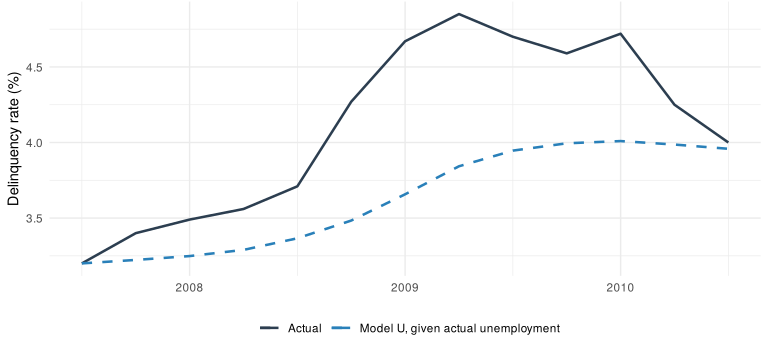
\includegraphics[width=0.85\textwidth]{figures/check2008.png}
\caption{Delinquency in the 2008 crisis: actual rate and rate implied by unemployment, 2007 Q3 to 2010 Q3}
\label{fig:check2008}
\note{Model U, estimated on the full sample, is given the actual change in unemployment from 2007 Q3. It explains 0.81 of the 1.65-point rise in delinquency up to the 2009 peak (49\%), and it rises later than the actual rate, because the crisis started in mortgage and consumer credit before it reached the labour market. This ratio is used in the main text to scale the severely adverse scenario.}
\end{figure}

\begin{table}[H]
\centering
\caption{Unemployment paths of the Fed's 2026 scenarios and forecast delinquency (\%)}
\label{tab:scenarios}
\small
\begin{tabular}{lcccc}
\toprule
 & \multicolumn{2}{c}{Baseline} & \multicolumn{2}{c}{Severely adverse} \\
\cmidrule(lr){2-3}\cmidrule(lr){4-5}
Quarter & Unemployment & Delinquency & Unemployment & Delinquency \\
\midrule
2026 Q1 & 4.6 & 2.58 & 5.9 & 2.68 \\
2026 Q2 & 4.6 & 2.54 & 7.2 & 2.84 \\
2026 Q3 & 4.6 & 2.51 & 8.2 & 2.98 \\
2026 Q4 & 4.5 & 2.47 & 9.0 & 3.09 \\
2027 Q1 & 4.5 & 2.44 & 9.5 & 3.17 \\
2027 Q2 & 4.4 & 2.42 & 9.9 & 3.22 \\
2027 Q3 & 4.3 & 2.39 & 10.0 & \textbf{3.25} \\
2027 Q4 & 4.3 & 2.38 & 9.8 & 3.23 \\
2028 Q1 & 4.3 & 2.37 & 9.4 & 3.18 \\
2028 Q2 & 4.3 & 2.37 & 9.1 & 3.12 \\
2028 Q3 & 4.3 & 2.36 & 8.7 & 3.06 \\
2028 Q4 & 4.3 & 2.36 & 8.4 & 3.01 \\
2029 Q1 & 4.2 & 2.35 & 8.0 & 2.95 \\
\bottomrule
\end{tabular}
\note{Unemployment paths from the Fed's 2026 supervisory scenarios, starting from 4.5\% in 2025 Q4. Delinquency is forecast with Model U from its 2025 Q4 level of 2.62\%, with the COVID-19 dummies set to zero. Model U + S is not used because the Fed's rate cuts steepen the yield curve at the start of the scenario, which the model would read as a sign of recovery.}
\end{table}

\end{document}
